\columnbreak
\section*{\LARGE Log-normal distributions of synaptic weights in noise driven networks}

In cortical circuits the distribution of synaptic weights has been repeatedly reported to be a log-normal \cite{Song2005}. in which very few strong weights are embedded in a sea of small weights. A number of computational models address the . Typically the result . Here we are following a hypothesis that not much is needed.


\section*{Network model}

The network is thus completely noise driven and devoid of correlations.



\section*{Results}

\begin{center}\vspace{1cm}
  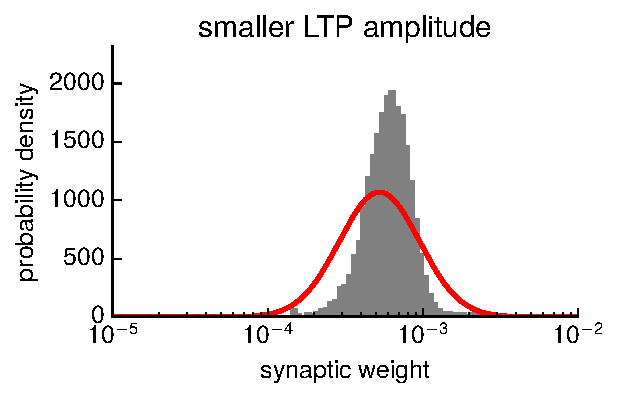
\includegraphics[width=.49\columnwidth]{%
    figures/syn_lnt_gnw_e07036_16.pdf}
  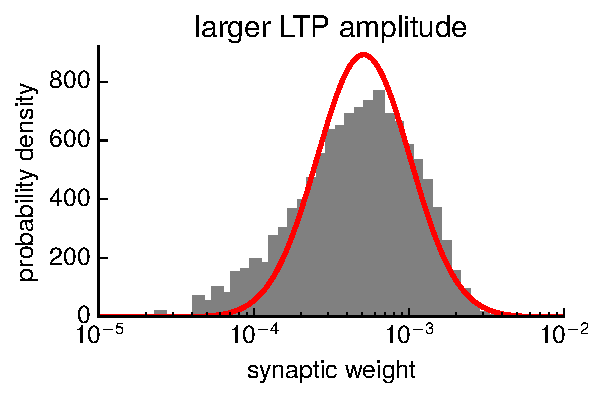
\includegraphics[width=.49\columnwidth]{%
    figures/syn_lnt_gnw_e07036_17.pdf}

  \captionof{figure}{}
\end{center}\vspace{1cm}


\begin{center}\vspace{1cm}
  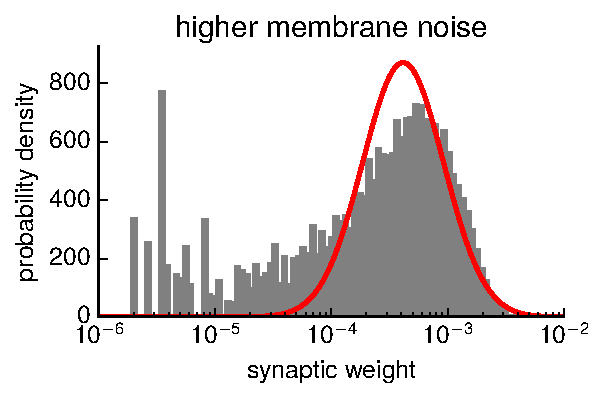
\includegraphics[width=.49\columnwidth]{%
    figures/syn_lnt_gnw_b20efe_0_highmem.pdf}
  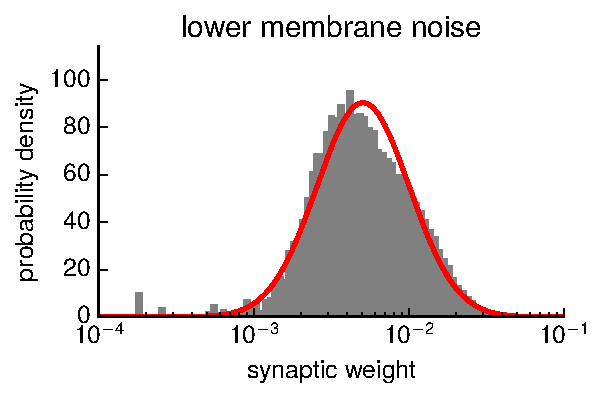
\includegraphics[width=.49\columnwidth]{%
    figures/syn_lnt_gnw_b20efe_0_lowmem.pdf}

  \captionof{figure}{$T=\text{\SI{900}{s}}$, LTD=-0.1 LTP}
\end{center}\vspace{1cm}


\section*{Coupled Networks}

